% LTeX: language=de_DE
\documentclass{uebung_cs}
\usepackage{algo223}
\usepackage{circuitikz}

\uebung{7}{}{}
\blattname{Übungen zu Woche 7: NP-Härte I}

\usepackage[ruled]{algorithm2e}

%%%%%%%%%%%%%%%%%%%%%%%%%%%%%%%%%%%%%%%%%%%%%%%%%%%%%%%%%%%%%%%%%%%%%%%%%%%%
\begin{document}
\section*{Dienstag}
\vspace{-1em}
Hinweis: Auf \href{https://moodle.studiumdigitale.uni-frankfurt.de/moodle/mod/questionnaire/view.php?id=241350}{Moodle} findet ihr eine Umfrage zu dieser Woche, bitte bis Montagabend ausfüllen.

\begin{exercise}[Schaltkreise][\athome\easy]
	% Eigenkreation
	In der Vorlesung haben wir eine Reduktion von \textsc{CircuitSat} auf \textsc{3SAT} gesehen.
	Welche \textsc{3CNF} Formel gibt diese Reduktion aus, wenn die Eingabe aus dem folgenden Schaltkreis besteht?
	%
	% \begin{figure}[ht]
	% 	\begin{center}
	% 		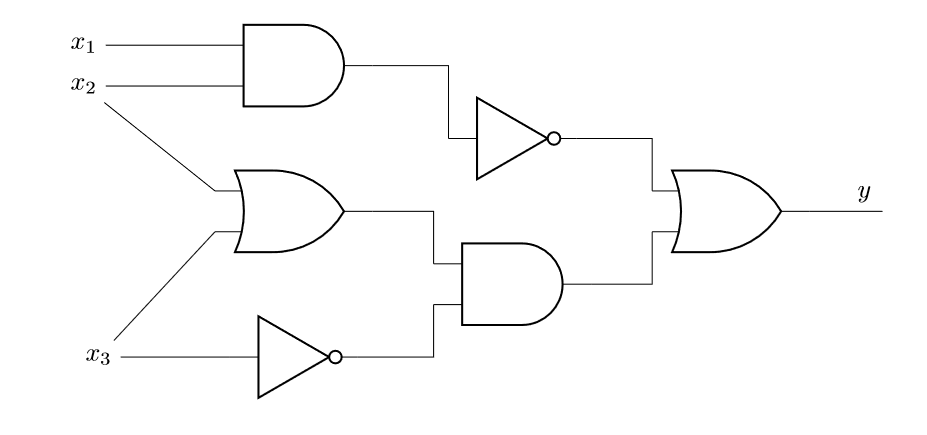
\includegraphics[scale=0.5]{schaltkreis}
	% 	\end{center}
	% \end{figure}
	\begin{figure}[ht]
		\begin{center}
			\begin{circuitikz}[scale=0.7,transform shape]
				\ctikzset{logic ports=ieee}
				\coordinate (branch2) at (-2,-1);
				\draw
				(0,2)  node[and port] (and_1) {}
				(0,0)  node[or port]  (or_1)  {}
				(0,-2) node[not port] (not_1) {}
				(3,1)  node[not port] (not_2) {}
				(3,-1) node[and port] (and_2) {}
				(6,0)  node[or port]  (or_2)  {}
				(and_1.out) -| (not_2.in)
				(or_1.out)  -| (and_2.in 1)
				(not_1.out) -| (and_2.in 2)
				(and_2.out) -| (or_2.in 2)
				(not_2.out) -| (or_2.in 1)
				(or_2.out) -- ++(1,0) node[near end,above]{\scalebox{1.428}{$z$}};

				\coordinate (In1) at ($ (and_1.in 1) + (-1.5,0) $);
				\coordinate (In2) at ($ (and_1.in 2) + (-1.5,0) $);
				\coordinate (In3) at ($ (or_1.in 2) + (-1.5,0) $);
				\node[left] at (In1) {\scalebox{1.428}{$x_1$}};
				\node[left] at (In2) {\scalebox{1.428}{$x_2$}};
				\node[left] at (In3) {\scalebox{1.428}{$x_3$}};

				% \coordinate (branch2) at (-2,1);
				\draw
				(In1) -| (and_1.in 1);

				\draw
				(In2) -| (and_1.in 2)
				(In2) -| (or_1.in 1);

				\draw
				(In3) -| (or_1.in 2)
				(In3) -| (not_1.in);

				% \draw[red]
				% (and_1.in 1) -- ++(-1.5,0)node[left](In11){\scalebox{1.428}{$x_1$}}
				% % (and_1.in 2) -- ++(-1.5,0)node[left](In2){\scalebox{1.428}{$x_2$}}
				% % (or_1.in 1) -- (In2)
				% (and_1.in 2) -- ++(-1.5,0)node[left](In22){\scalebox{1.428}{$x_2$}}
				% (or_1.in 1) -- (In2)
				% (not_1.in) -- ++(-1.5,0)node[left](In33){\scalebox{1.428}{$x_3$}}
				% (or_1.in 2) -- (In33);
			\end{circuitikz}
		\end{center}
	\end{figure}
\end{exercise}

\begin{exercise}[DNF Erfüllbarkeit][\athome]
	% Erickson, Chapter 12, Exercise 3
	Eine aussagenlogische Formel ist in \textit{disjunktiver Normalform} (DNF), wenn sie eine Disjunktion (\textsc{Or}) von Konjunktionstermen (\textsc{And}) ist. Ein Beispiel für eine DNF ist:
	$$(\overline{x} \wedge y \wedge \overline{z}) \vee (y \wedge z) \vee (x \wedge \overline{y} \wedge \overline{z}).$$
	Gegeben ist eine aussagenlogische Formel in disjunktiver Normalform. DNF-\textsc{Sat} entscheidet, ob diese Formel erfüllbar ist.
	\begin{enumerate}
		\item\easy Beschreibe einen Algorithmus, der DNF-\textsc{Sat} in Polynomialzeit  löst.
		\item\medium Wir zählen das Jahr 2050, Prof.\ Regloh steht kurz vor dem Ruhestand, das Institut für Informatik steht kurz vor dem Umzug auf den Campus Riedberg, und du stehst kurz vor deinem Studienabschluss. Prof.\ Regloh möchte am Ende seiner Forschungskarriere nochmal einen richtig großen Erfolg erzielen und hat sich schon seit ein paar Monaten psychisch auffällig verhalten. Jetzt rennt er jubelnd durch die Gänge, im Vorbeigehen schreit er dir folgendes zu:
		      \begin{quote}
			      Angenommen, wir haben eine aussagenlogische Formel in konjunktiver Normalform mit höchstens 3 Literalen pro Klausel. Wir wollen herausfinden, ob diese Formel erfüllbar ist. Wir können das Distributivgesetz für Boolesche Operationen verwenden, um eine äquivalente Formel in disjunktiver Normalform zu konstruieren. Zum Beispiel:
			      \[(x \vee y \vee \overline{z}) \wedge (\overline{x} \vee \overline{y}) \Leftrightarrow (x \wedge \overline{y}) \vee (y \wedge \overline{x}) \vee (\overline{z} \wedge \overline{x}) \vee (\overline{z} \wedge \overline{y})\,.\]
			      Nun können wir den Algorithmus aus Aufgabenteil a) verwenden, um in Polynomialzeit herauszufinden, ob die entstandene DNF erfüllbar ist. Wir haben also \textsc{3Sat} in Polynomialzeit gelöst! Da \textsc{3Sat} $\NP$-schwer ist, gilt $\P = \NP$! Ich werde eine Million Dollar als Preisgeld erhalten und berühmt werden!
		      \end{quote}
			  Stimmt sein Beweis? Begründe deine Antwort.%
			  \footnote{Hier ist eine Liste von 115 Manuskripten, die das P versus NP Problem mit derartigen oder ähnlich fehlerhaften Argumenten angeblich lösen: \url{https://www.win.tue.nl/~wscor/woeginger/P-versus-NP.htm}}
	\end{enumerate}
\end{exercise}
\newpage

\begin{exercise}[Interval Scheduling][\atschool]\
	% KT - Exercise 8.1
	% Entscheide für die beiden folgenden Fragen, welche der Antworten \enquote{Ja}, \enquote{Nein} oder \enquote{Unbekannt, da es $\P = \NP$ beantworten würde} zutrifft.
	Betrachte das folgende Entscheidungsproblem:
	\begin{quote}
		\textsc{IntervalScheduling}:\\
		Sei eine Menge von Intervallen auf einer Zeitleiste sowie eine Zahl~$k$ gegeben. Enthält diese Menge eine Teilmenge von sich nicht überschneidenden Intervallen der Größe mindestens~$k$?
	\end{quote}

	Im Folgenden schreiben wir $A \leq_p B$, wenn es eine Polynomialzeit-Reduktion gibt, die das Problem $A$ auf das Problem $B$ reduziert. Das heißt, das Problem $A$ soll in Polynomialzeit gelöst werden, falls es einen Algorithmus gibt, der $B$ in Polynomialzeit löst.
	\begin{enumerate}
		\item\medium Gilt \textsc{IntervalScheduling} $\leq_p$ \textsc{MaximumIndependentSet}? Begründe deine Antwort.\\\tipp{Modelliere Intervalle als Knoten. Was sind die Kanten?}
		\item\medium Gilt \textsc{MaximumIndependentSet} $\leq_p$ \textsc{IntervalScheduling}? Begründe deine Antwort.\\
		\tipp{Erinnere dich an Greedy-Algorithmen. Welche Konsequenzen hätte eine solche Reduktion?}
	\end{enumerate}
\end{exercise}


\begin{exercise}[Independent Set][\atschool]\
	% https://courses.engr.illinois.edu/cs374/fa2021/A/labs/lab12.pdf - Exercise 2
	Eine \emph{unabhängige Menge} in einem Graphen $G = (V,E)$ ist eine Teilmenge $S \subseteq V$, sodass $\{u,v\} \not\in E$ für alle $u,v \in S$ gilt. Betrachte die folgenden drei Probleme:

	\textsc{IndependentSet}: Gegeben ein Graph $G = (V,E)$ und eine Zahl $k \in \N$, gib \textsc{True} aus, wenn $G$ eine unabhängige Menge der Größe $k$ besitzt, sonst \textsc{False}.

	\textsc{MaximumIndependentSet}: Gegeben ein Graph $G = (V,E)$, gib die Größe der größten unabhängigen Menge in $G$ aus.

	\textsc{SearchMaximumIndependentSet}: Gegeben ein Graph $G = (V,E)$, gib eine unabhängige Menge in~$G$ mit maximaler Größe aus.

	Hierbei ist \textsc{IndependentSet} ein \emph{Entscheidungsproblem}, \textsc{MaximumIndependentSet} ist ein \emph{Optimierungsproblem} und \textsc{SearchMaximumIndependentSet} ist ein \emph{Suchproblem}.
	Wir zeigen nun, dass alle drei Problem äquivalent sind bezüglich Polynomialzeit-Reduktionen.
	\begin{enumerate}
		\item\easy
		Entwirf einen Polynomialzeit-Algorithmus~$A$ für \textsc{IndependentSet}, der einen hypothetischen Polynomialzeit-Algorithmus~$C$ für \textsc{SearchMaximumIndependentSet} als Subroutine benutzt.
		\item\medium 
		Entwirf einen Polynomialzeit-Algorithmus~$B$ für \textsc{MaximumIndependentSet}, der einen hypothetischen Polynomialzeit-Algorithmus~$A$ für \textsc{IndependentSet} als Subroutine benutzt.
		\item\hard
		Entwirf einen Polynomialzeit-Algorithmus~$C$ für \textsc{SearchMaximumIndependentSet}, der einen hypothetischen Polynomialzeit-Algorithmus~$B$ für \textsc{MaximumIndependentSet} als Subroutine benutzt.
		\tipp{Lösche immer einen Knoten und frag das Orakel~$B$}
		\item\medium
		Was wissen wir nun über alle drei Probleme, falls $\cc{P}\ne \cc{NP}$ gilt?
	\end{enumerate}
	%
	% \begin{itemize}[topsep=0.21cm, leftmargin=1.2cm]
	% 	\item \textsc{Input}: Ein ungerichteter Graph $G$ und eine Zahl $k \in \N$.
	% 	\item \textsc{Output}: \textsc{True}, wenn $G$ ein Independent Set der Größe $k$ besitzt, sonst \textsc{False}.
	% \end{itemize}
	% \begin{enumerate}
	% 	\item Benutze die Blackbox, um einen Algorithmus zu beschreiben, der folgendes Optimierungsproblem in Polynomialzeit löst:
	% 	      \begin{itemize}[topsep=0.21cm, leftmargin=1.2cm]
	% 		      \item \textsc{Input}: Ein ungerichteter Graph $G$.
	% 		      \item \textsc{Output}: Die Größe des größten Independent Set in $G$.
	% 	      \end{itemize}
	% 	\item Benutze die Blackbox, um einen Algorithmus zu beschreiben, der folgendes Suchproblem in Polynomialzeit löst:

	% 	      \begin{itemize}[topsep=0.21cm, leftmargin=1.2cm]
	% 		      \item \textsc{Input}: Ein ungerichteter Graph $G$.
	% 		      \item \textsc{Output}: Ein Independent Set in $G$ mit maximaler Größe.
	% 	      \end{itemize}
	% \end{enumerate}
\end{exercise}

\subsection*{Donnerstag}

\begin{exercise}[Search-to-Decision für 3SAT][\href{FF}{Moodle}\athome\medium]
	Angenommen es gibt einen Algorithmus $A$, der in Polynomialzeit für jede 3CNF-Formel~$\Phi$ entscheidet, ob diese erfüllbar ist.
	Konstruiere einen Polynomialzeit-Algorithmus~$B$, der~$A$ als Subroutine nutzt, um eine erfüllende Belegung von~$\Phi$ zu berechnen.
\end{exercise}

\begin{exercise}[Perfektes Matching][\atschool]
	% https://courses.engr.illinois.edu/cs374/fa2021/A/labs/lab12.pdf - Exercise 1
	Sei $G = (V,E)$ ein ungerichteter Graph. Eine Teilmenge $M \subseteq E$ ist ein \textit{Matching}, wenn keine zwei Kanten aus $M$ mit demselben Knoten verbunden sind. Ein Matching ist \textit{perfekt}, wenn jeder Knoten $v \in V$ zu einer Kante $m \in M$ inzident ist. Eine äquivalente Definition betrachtet die Größe des Matchings: $M$ ist perfekt genau dann, wenn $|M| = |V|/2$ gilt. Wir definieren das \textsc{PerfectMatching}-Problem:
	\begin{quote}
		\textsc{PerfectMatching}:\\
		Gegeben sei ein ungerichteter Graph $G = (V,E)$. Existiert ein perfektes Matching in $G$?
	\end{quote}
	Dieses Problem kann in Polynomialzeit gelöst werden. Für allgemeine Graphen handelt es sich hierbei um einen recht komplizierten Algorithmus, der einen Meilenstein in der kombinatorischen Optimierung darstellt, und viele Anwendungen in Theorie und Praxis hat.
	Auf bipartiten Graphen ist das Problem einfacher zu lösen:
	\begin{enumerate}
		\item\medium Entwirf einen Polynomialzeit-Algorithmus für \textsc{PerfectMatching} auf bipartiten Graphen.\\\tipp{Flussnetzwerk}
	\end{enumerate}
	% Ein Graph $G = (V,E)$ ist \textit{bipartit}, wenn die Knoten auf zwei disjunkte Teilmengen~$L$ und~$R$ verteilt werden können, sodass alle Kanten zwischen $L$ und $R$ liegen. In anderen Worten: $L$ und $R$ sind jeweils unabhängige Knotenmengen (\textit{independent set}).
	Prof.\ Regloh behauptet, dass der folgende Algorithmus das Problem von allgemeinen Graphen auf bipartite Graphen reduziert:
	\begin{quote}
		\textsc{ReduceGraph}$(G)$:\\
		Gegeben sei ein ungerichteter Graph $G = (V,E)$. Erstelle daraus einen bipartiten Graphen $H = (V \times \{1,2\},E_H)$ wie folgt:\\
		Jeder Knoten $u \in V$ wird zu zwei Kopien $(u,1)$ und $(u,2)$. Die Knotenmenge von~$H$ ist also partitioniert in zwei disjunkte Teile $V_1$ und $V_2$ eines bipartiten Graphen, wobei
		\begin{equation*}
			V_1 = \{(u,1)\,|\,u\in V\}\ \text{ und }\ V_2 = \{(u,2)\,|\,u\in V\}\,.
		\end{equation*}
		Die Menge $E_H$ der Kanten von~$H$ ist definiert via
		\[E_H = \Big\{\;\{(u,1),(v,2)\}\,\;\Big|\;\,\{u,v\} \in E\;\Big\}\,.\]
		Mit anderen Worten: Für alle Kanten $\{u,v\}$ auf~$G$ fügen wir eine Kante zwischen $(u,1)$ und $(v,2)$ in~$H$ ein. Beachte, dass~$G$ keine Eigenschleifen hat und es dadurch in $H$ für alle $u \in V$ keine Kante  $\{(u,1),(u,2)\}$ geben kann.
	\end{quote}
	Ist die vorgeschlagene Reduktion korrekt? Um das herauszufinden, müssen wir überprüfen, ob $H$ genau dann ein perfektes Matching hat, wenn $G$ eins hat.
	\begin{enumerate}[resume]
		\item\medium Zeige die folgende Aussage: Wenn $G$ ein perfektes Matching hat, dann hat auch $H$ eins.
		\item\medium Widerlege die folgende Aussage: Wenn $G$ kein perfektes Matching hat, dann hat auch $H$ keins.
		      \begin{itemize}
			      \item Konstruiere ein Gegenbeispiel, in dem $G$ drei Knoten hat. \tipp{Dreieck}
			      \item Konstruiere ein Gegenbeispiel, in dem $G$ eine gerade Anzahl an Knoten hat.
		      \end{itemize}
			  Begründe jeweils, warum die behauptete Implikation falsch ist.
	\end{enumerate}
\end{exercise}

\clearpage
\section*{Optionale Aufgaben und Projekte}

\begin{exercise}[Kundenanalyse][\hard]
	% KT - Exercise 8.2
	Zur Analyse des Kundenverhaltens benutzen Geschäfte oftmals ein zweidimensionales Array $A$, in dem jede Zeile zu einem Kunden und jede Spalte zu einem verkauften Produkt korrespondiert. Ein Eintrag $A[i,j]$ gibt an, welche Menge von Produkt $j$ der Kunde $i$ gekauft hat, so hat Chelsea im folgenden Beispiel siebenmal Katzenstreu gekauft:

	\begin{center}
		\begin{tabular}{l c c c c}
			\hline
			        & Waschmittel & Bier & Windeln & Katzenstreu \\
			\hline
			Raj     & 0           & 6    & 0       & 3           \\
			Alanis  & 2           & 3    & 0       & 0           \\
			Chelsea & 0           & 0    & 0       & 7           \\
			\hline
		\end{tabular}
	\end{center}

	Ein Geschäft möchte nun zur Marktforschung eine \textit{diverse} Teilmenge der Kunden finden. Eine Teilmenge $S$ der Kunden heißt \textit{divers}, wenn keine zwei Kunden aus $S$ jemals dasselbe Produkt gekauft haben (das heißt, es gibt für jedes Produkt nur genau einen Kunden aus $S$, der es gekauft hat). Nun lässt sich das folgende Entscheidungsproblem formulieren:
	\begin{quote}
		\textsc{DiverseTeilmenge}:\\
		Seien ein $n \times m$ Array $A$, wie oben definiert, und eine natürliche Zahl $k$ mit $k \leq n$ gegeben. Gibt es eine \textit{diverse} Teilmenge $S$ der Kunden mit $|S| \geq k$?
	\end{quote}
	Zeige, dass \textsc{DiverseTeilmenge} \NP-vollständig ist.
\end{exercise}

% \begin{exercise}[Feriencamp]
% 	% KT - Exercise 8.3
% 	Bei der Organisation eines Feriencamps wirst du mit dem Problem \textsc{EffizientesRekrutieren} konfrontiert.
% 	\begin{quote}
% 		\textsc{EffizientesRekrutieren}:\\
% 		Für jede der $n$ im Feriencamp angebotenen Sportarten muss es einen für diesen Sport geschulten Betreuer geben. Es haben sich $m$ potenzielle Betreuer beworben. Für jede der $n$ Sportarten gibt es eine Teilmenge der $m$ Bewerber, die für diese Sportart qualifiziert sind. Ist es möglich, maximal $k < m$ Betreuer einzustellen, sodass mindestens ein Betreuer für jede Sportart geschult ist?
% 	\end{quote}	 

% 	Zeige, dass \textsc{EffizientesRekrutieren} \NP-vollständig ist.
% \end{exercise}

\begin{exercise}[Search-to-Decision für 3COLOR][\hard]
	Angenommen es gibt einen Algorithmus $A$, der in Polynomialzeit für jeden Graphen~$G$ entscheidet, ob dieser eine echte Knotenfärbung mit drei Farben zulässt.
	Konstruiere einen Polynomialzeit-Algorithmus~$B$, der~$A$ als Subroutine nutzt, um eine solche echte Färbung zu konstruieren.
	(Hinweis: $A$ darf wirklich nur ungefärbte Graphen als Eingabe erhalten.)
\end{exercise}

% \begin{exercise}[Search-to-Decision]\
% 	% Erickson, Chapter 12, Exercise 5b,c,d
% 	\begin{enumerate}
% 		\item Du besitzt eine magische Blackbox, die in Polynomialzeit herausfindet, wie viele Knoten ein größter vollständiger Teilgraph ein beliebiger Graph $G$ besitzt. Beschreibe und analysiere einen Algorithmus, der in Polynomialzeit für einen beliebigen Graphen $G$ einen vollständigen Teilgraphen maximaler Größe berechnet. Benutze dafür die Blackbox.
		
% 		\item Ein ungerichteter Graph $G$ heißt $3$-färbbar, wenn es eine Funktion $c:V(G)\to\{\texttt{R},\texttt{G},\texttt{B}\}$ gibt, die jedem Knoten eine von drei Farben zuordnet, sodass benachbarte Knoten unterschiedliche Farben erhalten (siehe erster Absatz in Erickson 12.10).

% 		      Du besitzt eine magische Blackbox, die in Polynomialzeit herausfindet, ob ein beliebiger Graph $G$ $3$-färbbar ist. Beschreibe und analysiere einen Algorithmus, der in Polynomialzeit für einen beliebigen Graphen $G$ eine richtige $3$-Färbung ausgibt oder richtigerweise ausgibt, dass keine solche Färbung existiert. Benutze dafür die Blackbox.\\
% 		      \textit{Tipp: Die Eingabe für die Blackbox ist ein Graph und nichts Anderes.}

% 		\item Du besitzt eine magische Blackbox, die in Polynomialzeit herausfindet, ob eine beliebige Boolesche Formel $\Phi$ erfüllbar ist (zum Beispiel $\Phi= (x \Leftrightarrow ((z\wedge y)\vee \overline{x})) \wedge (y \Rightarrow \overline{x})$). Beschreibe und analysiere einen Algorithmus, der in Polynomialzeit eine erfüllende Belegung der Variablen von $\Phi$ ausgibt, oder richtigerweise ausgibt, dass so eine Belegung nicht existiert. Benutze dafür die Blackbox.
% 	\end{enumerate}
% \end{exercise}

\end{document}
